\section*{Introduction}
A field-effect transistor (FET) is a type of transistor that uses an electric field to control the flow of current in a semiconductor. It gas two types -- junction FET (JFET) and metal-oxide-semiconductor FET (MOSFET). 

A Metal Oxide Semiconductor Field-effect Transistor (MOSFET) is a FET with an insulated gate. It has 4 terminals -- source (S), gate (G), drain (D) and body (B). In general, the body of the MOSFET is in connection with the source terminal thus forming a three-terminal FET. The charge carriers enter into the channel through the source terminal and exit via the drain through a channel whose width is controlled by the voltage on an electrode which is called the gate and it is located in between the source and the drain. It is insulated from the channel by an extremely thin layer of metal oxide.

\begin{figure}[H]
    \centering
    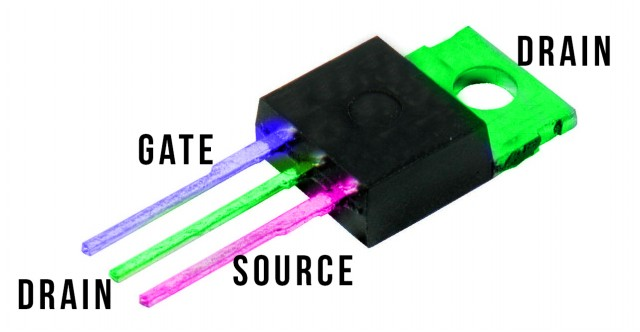
\includegraphics[width=0.4\columnwidth]{images/real.jpg}
    \caption{A typical MOSFET structure}
\end{figure}

\section*{Working Principle}

\begin{figure}[H]
    \centering
    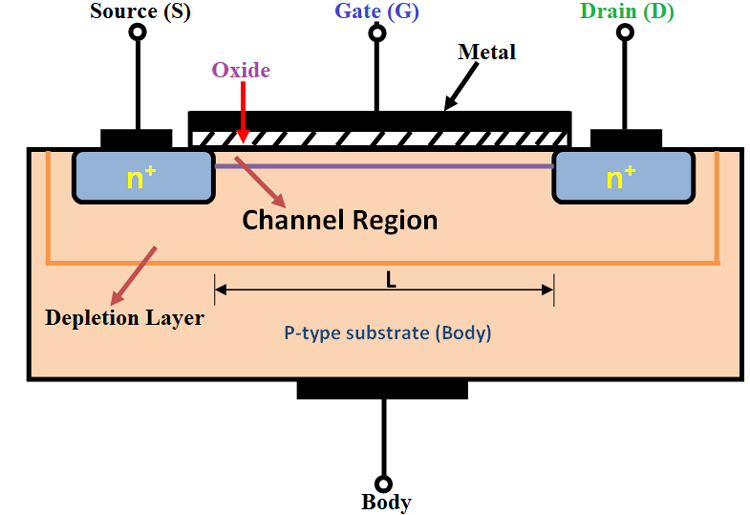
\includegraphics[width=0.55\columnwidth]{images/str.png}
    \caption{Internal structure of a N-channel enhancement type MOSFET}
    \label{str}
\end{figure}

Fig. \ref{str} shows the internal structure of a MOSFET. The source (S) and drain (D) regions are heavily doped n-type semiconductors and between them, the body (B) is a p-type semiconductor. There is a thin layer of metal oxide i.e. a dielectric which creates the gate terminal (G).

If we connect a voltage source between D and S, $V_{ds}$, it increases the potential at the drain terminal, thus increasing the depletion region between the drain and the body. Due to this, there will be no current flow from the drain to the source and the MOSFET is off. This is also called the \textbf{cutoff region}.

To flow current from drain to source, we need to create a channel between them. We can connect a voltage source $V_{gs}$ between the gate and the source. Since the body is a p-type semiconductor, the electrons being the minority charge carriers accumulate near the gate. This acts as a capacitive layer. As we keep on increasing $V_{gs}$, the electrons start filling the holes near the gate and holes start moving away from the gate. Hence due to this electrons, the region near the gate acts as a channel between the source and the drain such that electrons can move from the source to the drain. The voltage at which the channel is formed is called the \textbf{threshold voltage}. As the conventional current flows from drain to the source, it is called \textbf{drain current}. This region is also called the \textbf{ohmic region}. The width of the channel is controlled by $V_{gs}$.

However, as the voltage $V_{ds}$ increases, the depletion layer between the drain and the body will increase as they are reverse biased. Also the channel begins to deplete towards the drain end since the drain is at a positive potential and negative charges from the channel closest to the drain are being pulled into the drain. This reduces the width of the channel, also known as the \textbf{pinch-off effect}. Practically the flow is not completely pinched off due to the large flow of electrons in the channel, and instead there is a constant saturated current. The voltage at which the current saturates is called the \textbf{saturation voltage} and this region is called the \textbf{saturation region}.

\begin{figure}[H]
    \centering
    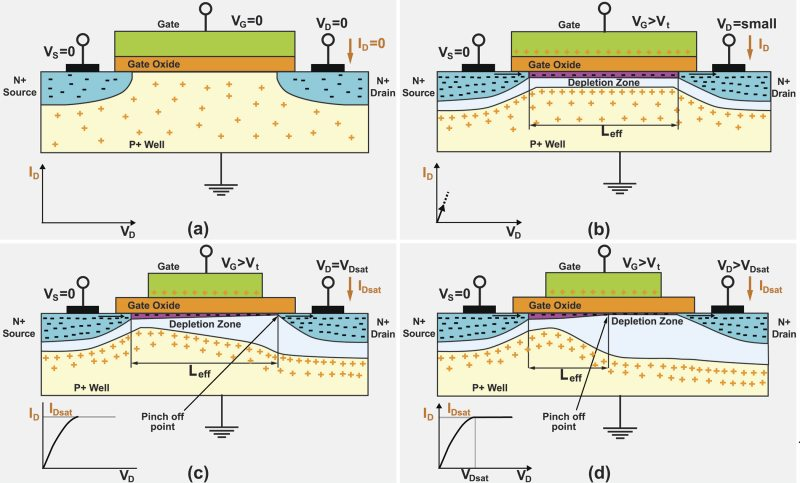
\includegraphics[width=1\columnwidth]{images/stages.jpg}
    \caption{Operating stages of an N-channel enchancement MOSFET}
    % \label{drain}
\end{figure}

To increase the saturation current, one can control the gate voltage $V_{gs}$, since it controls the width of the channel. Fig. \ref{drain} and \ref{trans} show the corresponding drain and transfer characterstics of this MOSFET.

\begin{figure}[H]
    \centering
    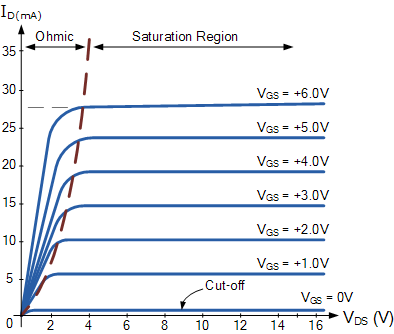
\includegraphics[width=0.58\columnwidth]{images/drain.png}
    \caption{Typical $i_d$ vs. $v_{ds}$ characterstic curve for different values of $v_{gs}$}
    \label{drain}
\end{figure}

\begin{figure}[H]
    \centering
    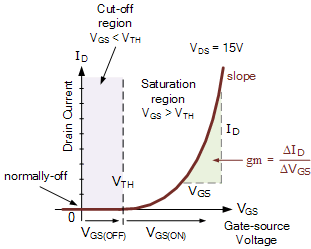
\includegraphics[width=0.5\columnwidth]{images/trans.png}
    \caption{Transfer characteristics of the MOSFET with a fixed $v_{ds}$}
    \label{trans}
\end{figure}

With a fixed $v_{ds}$ drain-source voltage connected across the MOSFET we can plot the values of drain current, $i_ds$ with varying values of $v_{gs}$ to obtain a graph of the forward DC characteristics. The gain of the MOSFET can be written as,

\begin{align*}
    \text{Gain } &= \frac{i_{ds}}{i_{gs}}\\
    \text{where } i_{gs} &= \frac{v_{gs}}{X_C} = v_{gs}\cdot 2\pi f C_{ox}\\
    i_{ds} &= g_m\,v_{gs}
\end{align*}

Here $g_m$ is the transconductance of the transistor which is short for “transfer conductance” and has the unit of Siemens (S) (or A V$^{-1}$). Voltage gain of a mosfet amplifier is directly proportional to the transconductance and to the value of the drain resistor.

\begin{align}
    \text{Gain } &= \frac{g_m}{2 \pi f C_{ox}} \label{gain}
\end{align}

% ======================================================================================
\subsection*{Frequency Response}
One can see from Eq. \ref{gain} that $f \propto 1/C_{ox}$. 
The value of $C_{ox}$ comes from the capacitive layer formed by the overlap between the source-gate and drain-gate terminals.

\begin{align*}
    C_{ox} = C_{gs} \cdot W \cdot (L+\Delta L)
\end{align*}

Here, $C_{gs}$ is the capacitance per unit area and and $W$ and $L$ refer to the width and length of the configuration. $\Delta L = 0$ can be achieved by not overlapping the gate with the source and drain terminals. $L$ is typically in the order of nanometers currently. Since $C_{gs}$ is proportional to the charge induced, it can only be minimized to an extent as it also determines the distinction between the ON and OFF state of the MOSFET.

% ======================================================================================
\section*{Advantage over BJTs}
A BJT requires current to be applied to the base terminal, which requires energy.
MOSFETs, also called voltage controlled devices, only require voltage at the gate to control the amount of current from the drain to source. Hence almost no current flows, which makes them more efficient. MOSFETs can also handle much more currents than typical BJTs.

MOSFETs also have higher input impedance, lower on-resistance and are less sensitive to temperatures.

\section*{Types}
The previous sections particularly describes the working principle of the N-channel \textbf{enhancement type} MOSFET. There is also the \textbf{depletion type} MOSFET where the channel is present by default and thus they require a negative voltage to turn off (i.e. they are normally on as opposed to enhancement type which is normally off). The there is further division into \textbf{N-channel} and \textbf{P-channel} for both the categories, where the p and n type semiconductors as well as the roles of holes and electrons are reversed.

\begin{figure}[H]
    \centering
    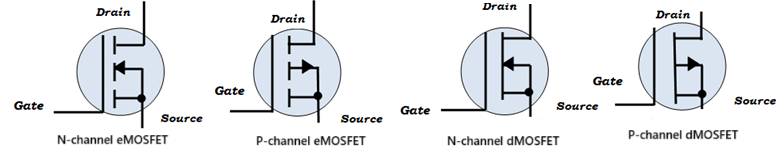
\includegraphics[width=1\columnwidth]{images/types1.png}
    \caption{Circuit symbols of all 4 kinds of MOSFETs}
\end{figure}

\section*{Applications}
MOSFETs are widely used instead of BJTs because they are faster, more efficient, more temperature-stable, and easier to drive. Some They are widely used as switches as they can switch on and off very fast, which allows it to handle high frequencies and reduce power losses. They are used as high-frequency amplifiers and can perform various functions such as chopping, regulating, sensing, processing, etc.